%TC:envir minted 1 xall 
%TC:envir algorithmic 1 xall

% Include tables in word count
%TC:envir table 0 word
%TC:envir tabular 1 word

% Include footnotes in word count
%TC:macro \footnote [text]
%TC:macro \footnotetext [text]

%TC:group minted 0 0
%TC:macro \mintinline [ignore]
%TC:macro \colb [ignore]
%TC:macro \hyperref [ignore]

You will need three Raspberry Pis: two acting as hosts and one as the router. You will also need two Ethernet cables and two USB-to-Ethernet adapters. Use the cables to connect both your hosts to the router as shown below. Static router addresses have been defined by the P4 program.

\begin{figure}[htbp]
  \centering
    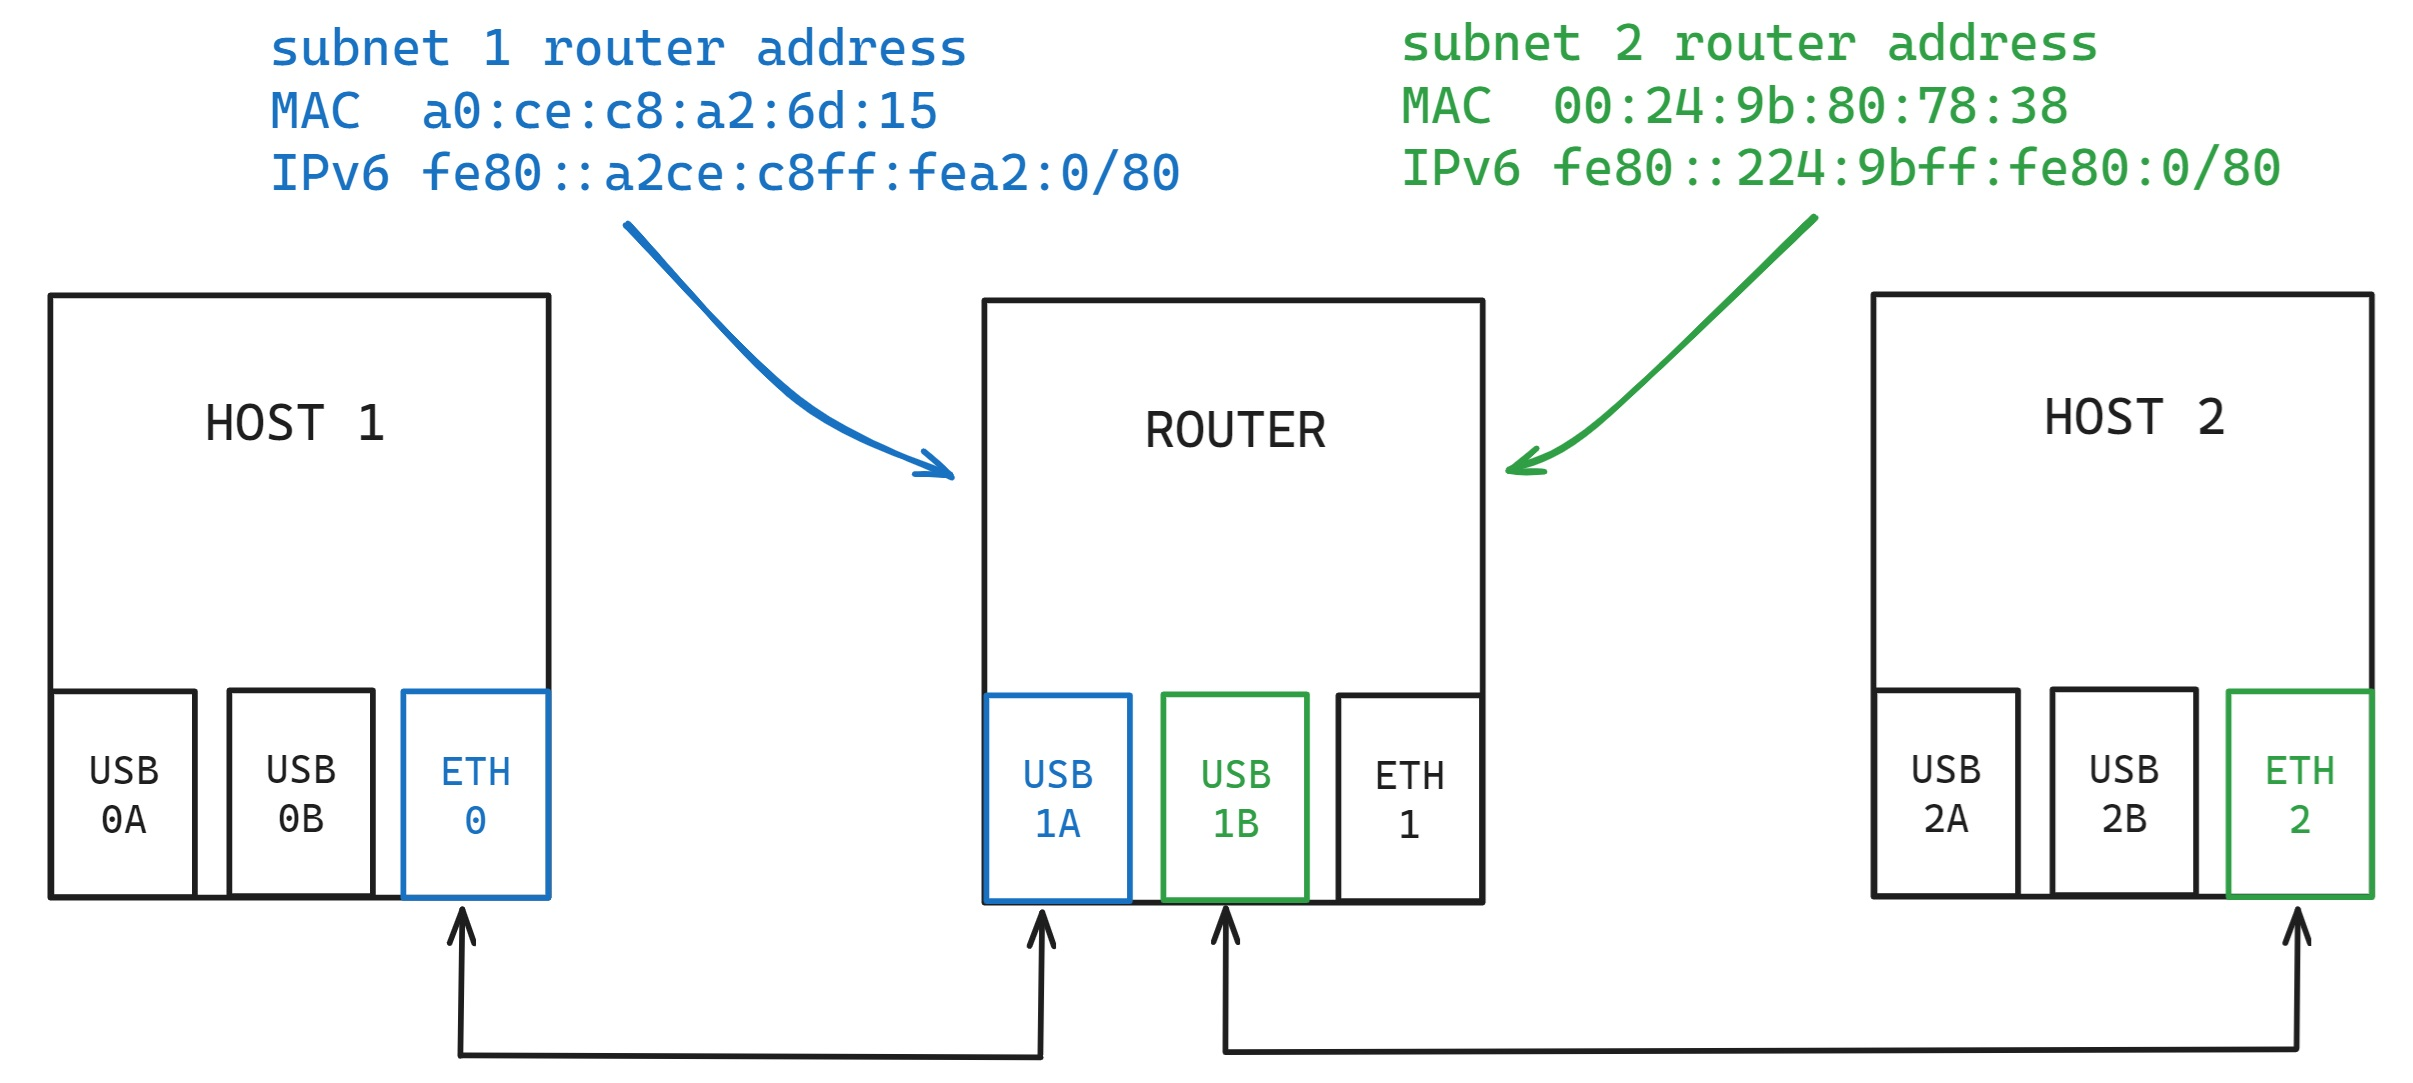
\includegraphics[width=1\textwidth]{figures/appendices/icmpv6_ndp_setup.jpg}
\end{figure}

Run \texttt{ip a} on the router to learn the MAC and IP addresses of the USB ports connected to your hosts. Edit the P4 program to define constant static router IPv6 and MAC addresses (at the top of the program) such that you have one entry for each subnet. These will be referred to as \texttt{IPra}, \texttt{MACra} and \texttt{IPrb}, \texttt{MACrb}. The MAC addresses should match the router’s port MAC addresses, and the IP addresses should belong to the same subnets as the ports. 

Choose IPv6 addresses \texttt{IPa} and \texttt{IPb} for the hosts such that they belong to the same subnet as their respective router USB ports. Also run \texttt{ip a} on the hosts to learn their MAC addresses \texttt{MACa} and \texttt{MACb}.

On Host 1, open a command prompt and run:
\begin{quote}
    \texttt{sudo ifconfig eth0 inet6 add IPa}
    
    \texttt{sudo ip -6 route add dev eth0 IPra}
    
    \texttt{sudo ip -6 neigh show}
\end{quote}

The first line sets a static IPv6 address on Host 1 and the second line defines a route to the static address. The third line prints out all entries in the host’s neighbour table. It should be initially empty.

Start the P4 program on the router using the port connected to Host 1. Start up the CLI and enter the commands (or run these by using a \texttt{commands.txt} file, as explained in Appendix A):
\begin{quote}
    \texttt{table\_add MyIngress.nei\_responder MyIngress.nei\_adv IPa => MACa 1}
    
    \texttt{table\_add MyIngress.nei\_responder MyIngress.nei\_adv IPb => MACb 2}
    
    \texttt{table\_add MyIngress.nei\_responder MyIngress.nei\_adv IPra => MACra 1}
    
    \texttt{table\_add MyIngress.nei\_responder MyIngress.nei\_adv IPrb => MACrb 2}
\end{quote}

Then, run the \texttt{ping} command on Host 1:
\begin{quote}
    \texttt{ping6 -I eth0 IPra}
\end{quote}
This should not generate any response, as no Echo Reply functionalities have been written into the program. Finally, run:
\begin{quote}
    \texttt{sudo ip -6 neigh show}
\end{quote}

There should now be an entry associating \texttt{IPra} with \texttt{MACra}. Pinging Host 2 should add another entry to the neighbour table. The same commands can be performed on Host 2 to acquire the MAC addresses of the router and Host 1.
